\documentclass[12pt]{article}

\usepackage{graphicx}
\usepackage{amsmath}
\usepackage{amssymb}
\usepackage{natbib}
\usepackage{amsfonts}
\usepackage{multicol}
\usepackage{float}
\usepackage{oldgerm}
\usepackage{bm}
\usepackage{mathtools}
\usepackage{wrapfig}
\usepackage{fancyhdr}
\usepackage[export]{adjustbox}
\usepackage{xcolor}

\pagestyle{empty}

\newcommand{\Avec}{\mathbf A}
\newcommand{\Bvec}{\mathbf B}
\newcommand{\Dvec}{\mathbf D}
\newcommand{\Evec}{\mathbf E}
\newcommand{\Fvec}{\mathbf F}
\newcommand{\Jvec}{\mathbf J}
\newcommand{\Lvec}{\mathbf L}
\newcommand{\Mvec}{\mathbf M}
\newcommand{\Pvec}{\mathbf P}
\newcommand{\Rvec}{\mathbf R}
\newcommand{\Svec}{\mathbf S}
\newcommand{\Tvec}{\mathbf T}
\newcommand{\avec}{\mathbf a}
\newcommand{\bvec}{\mathbf b}
\newcommand{\dvec}{\mathbf d}
\newcommand{\evec}{\mathbf e}
\newcommand{\fvec}{\mathbf f}
\newcommand{\jvec}{\mathbf j}
\newcommand{\kvec}{\mathbf k}
\newcommand{\nvec}{\mathbf n}
\newcommand{\pvec}{\mathbf p}
\newcommand{\rvec}{\mathbf r}
\newcommand{\svec}{\mathbf s}
\newcommand{\vvec}{\mathbf v}
\newcommand{\xvec}{\mathbf x}
\newcommand{\yvec}{\mathbf y}
\newcommand{\zvec}{\mathbf z}
\newcommand{\nablav}{\boldsymbol{\nabla}}
\newcommand{\nablavector}{\vec \nabla}
\newcommand{\alphavec}{\boldsymbol{\alpha}}
\newcommand{\phivec}{\boldsymbol{\phi}}
\newcommand{\thetavec}{\boldsymbol{\theta}}
\newcommand{\omegavec}{\boldsymbol{\omega}}
\newcommand{\tauvec}{\boldsymbol{\tau}}
\newcommand{\ezero}{\varepsilon_{0}}
\newcommand{\mzero}{\mu_{0}}
\newcommand{\mubold}{\boldsymbol{\mu}}
\newcommand{\uniti}{\hat{\boldsymbol{\imath}}}
\newcommand{\unitj}{\hat{\boldsymbol{\jmath}}}
\newcommand{\unitk}{\hat{\boldsymbol{\mathit{k}}}}
\newcommand{\unitn}{\hat{\mathbf n}}
\newcommand{\unitr}{\hat{\mathbf r}}
\newcommand{\unitphi}{\hat{\boldsymbol{\phi}}}
\newcommand{\unittheta}{\hat{\boldsymbol{\theta}}}

\newcommand{\bit}{\begin{itemize}}
\newcommand{\eit}{\end{itemize}}

\setlength{\headsep}{0.5cm}
\setlength{\oddsidemargin}{-0.5cm}
\setlength{\textwidth}{16.5cm}
\setlength{\textheight}{24cm}
\voffset = -2cm

\pagestyle{fancy}
\fancyhf{}
\rfoot{
\includegraphics[width=1.0in]{cnm.png}}
\lfoot{ENGR 2910 Homework 10}
\begin{document}

%{\bf \underline{STUDENT NAME}:} 
%\vspace{1cm}

\begin{center}
\hfil
%\begin{wrapfigure}{l}{0.5in} 
%    
\includegraphics[width=0.5in]{cnm.png}
%\end{wrapfigure}
{\large\bf {ENGR 2910-101: Circuit Analysis}}
\hfill Instructor: Leo Silbert \\
Homework 10: 11/10/21 \hfill Due: 11/17/21\\
\hrulefill\\
\end{center}

%{\em Show all your working to ensure you obtain full points. Partial
%  credit will be given for correct algebraic steps if you fail to
%  obtain the correct final answer.}\\

%\newpage


\noindent
{\bf Question 1} [10]

The current in a 20 mH inductor is
\begin{align*}
i &= 40~\text{ mA }, & t \leq 0\\
i(t) &=  ( A_{1} e^{-10000 t} + A_{2} e^{-40000 t} ) \text{ A }, & t \geq 0.
\end{align*} 
At $t=0$, the voltage across the inductor is 28 V.

Find the expresion for the voltage across the inductor for $t>0$.

\newpage
\noindent
{\bf Question 2} [10]

For $t<0$, the current in the inductor is 1 A in the circuit below. The inductor voltage for $t>0$ is given by,
\begin{align*}
v_{L}(t) & = 3 e^{-4t} \text{ mV }, & 0^{+} \leq t \leq 2 \text{ s }\\
 v_{L}(t) &= - 3 e^{-4(t-2)} \text{ mV }, & 2 \leq t < \infty \text{ s }.
\end{align*}
\begin{figure}[h!]
     \centering
\vspace{-0.2in}
     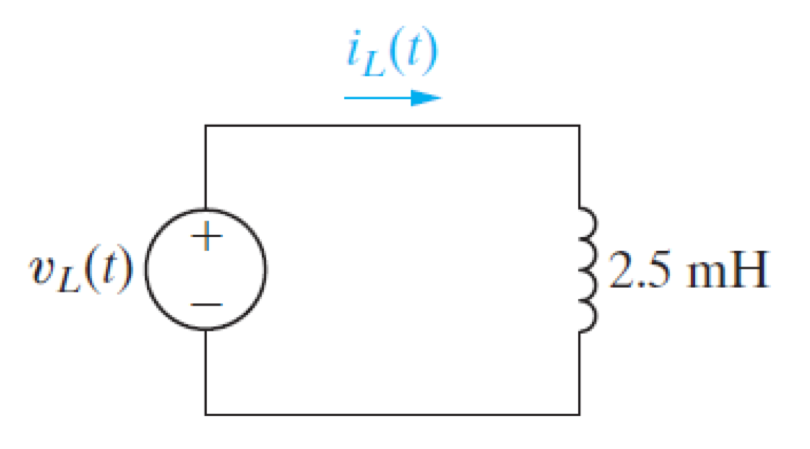
\includegraphics[clip,width=0.4\textwidth]{Fig6-11.png}
\vspace{-0.15in}
\end{figure}

Calculate the current $i_{L}(t)$ for the entire period $ 0 \leq t < \infty$ and sketch, {\bf by hand}, both $v_{L}(t)$ and $i_{L}(t)$. 

\newpage
\noindent
{\bf Question 3} [10]

At the moment the switch is opened in the circuit below, there is no energy stored in the inductor. 
$L_{1} = 5$H, $L_{2} = 0.2$ H, $M = 0.5$ H, and $R_{o} = 10 \Omega$.
\begin{figure}[h!]
  \centering 
  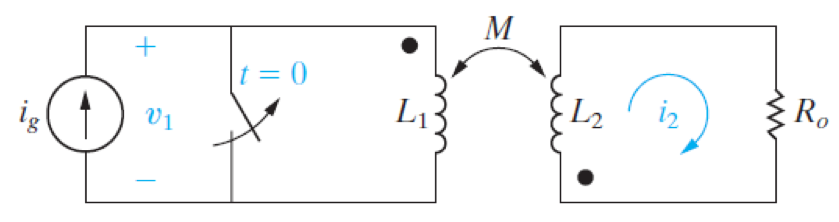
\includegraphics[clip,width=0.7\textwidth]{Fig6-41.png}
\end{figure}

\bit

\item[(i)]

Derive the differential equation that governs the behavior of $i_{2}$.

\item[(ii)]

If, $i_{g} = (e^{-10t} - 10)$ A for $t \geq 0$ and $i_{2}(t) = (625 e^{-10t} - 250 e^{-50 t}$) mA, what is the expression for the voltage, $v_{1}$, across the current source?
\eit

\newpage
\noindent
{\bf Question 4} [10]

For the following circuit:
\begin{figure}[h!]
  \centering 
  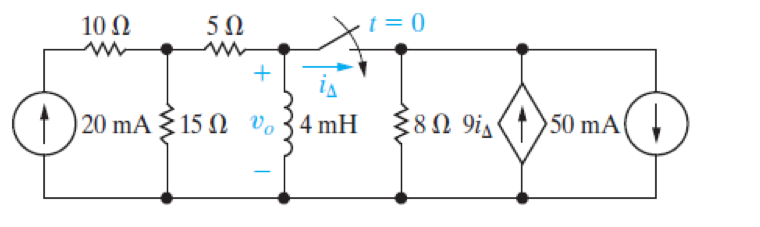
\includegraphics[clip,width=0.8\textwidth]{Fig7-44.png}
\end{figure}

\bit

\item[(i)]

Analyze the $t<0$ circuit to find the initial current flowing through the inductor.

\item[(ii)]

Analyze the $t = 0^{+}$ circuit. Perform a node analysis to arrive at an equation for the voltage across the $15 \Omega$ resistor in terms of $v_{o}$.

\item[(iii)]

Similarly, perform a node analysis at the inductor node to arrive at an equation for $i_{\Delta}$, and hence compute the initial voltage $v_{o}(0^{+})$. 

\eit

\newpage
\noindent
{\bf Question 5} [10]

The voltage source for the circuit in (a) is shown in (b). There is no energy stored in the capacitor for $t<0$. 
\begin{figure}[h!]
\centering 
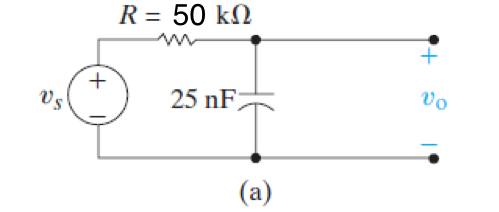
\includegraphics[clip,width=0.45\textwidth]{Fig7-83a.png}
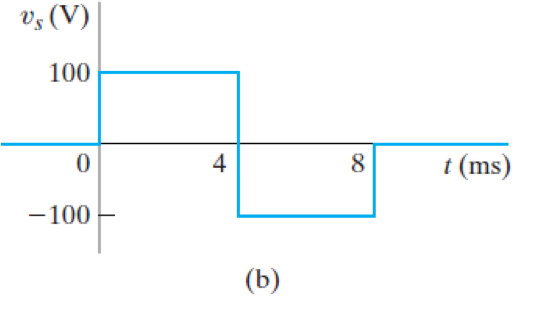
\includegraphics[clip,width=0.45\textwidth]{Fig7-83b.png}
\end{figure}

\bit

\item[(i)]

Derive the three expressions for $v_{o}(t)$ for the three time intervals: $0 \leq t \leq 4$ ms, 4 ms $\leq t \leq 8$ ms, and $t \geq 8$ ms.

\item[(ii)]

On the same figure, {\bf draw by hand}  $v_{o}$ and $v_{s}$. 

\eit

\end{document}
